\documentclass[tikz,border=8pt]{standalone}
% Shared look for every TikZ diagram. Load with \input{../../tools/tikz-style.tex}
\usepackage[T1]{fontenc}
\usepackage{lmodern}
\renewcommand{\sfdefault}{lmr}  % diagrams use the same serif as the text
\usetikzlibrary{arrows.meta, positioning, shapes.geometric, calc, fit, backgrounds}
\definecolor{cblue}{HTML}{4C78A8}
\definecolor{corange}{HTML}{F58518}
\definecolor{cgreen}{HTML}{54A24B}
\definecolor{cred}{HTML}{E45756}
\definecolor{cpurple}{HTML}{B279A2}
\definecolor{cgrey}{HTML}{6B6B6B}
\tikzset{
  every picture/.style={font=\sffamily, line width=1.2pt},
  box/.style={draw=#1, fill=#1!12, rounded corners=4pt, align=center, inner sep=7pt, minimum height=1.1cm},
  box/.default=cgrey,
  arrow/.style={-{Stealth[length=3mm]}, draw=cgrey, line width=1.4pt},
  title/.style={font=\sffamily\bfseries\Large},
  note/.style={font=\sffamily\small, text=cgrey, align=center},
}
\AtBeginDocument{\hyphenpenalty=10000 \exhyphenpenalty=10000}

\begin{document}
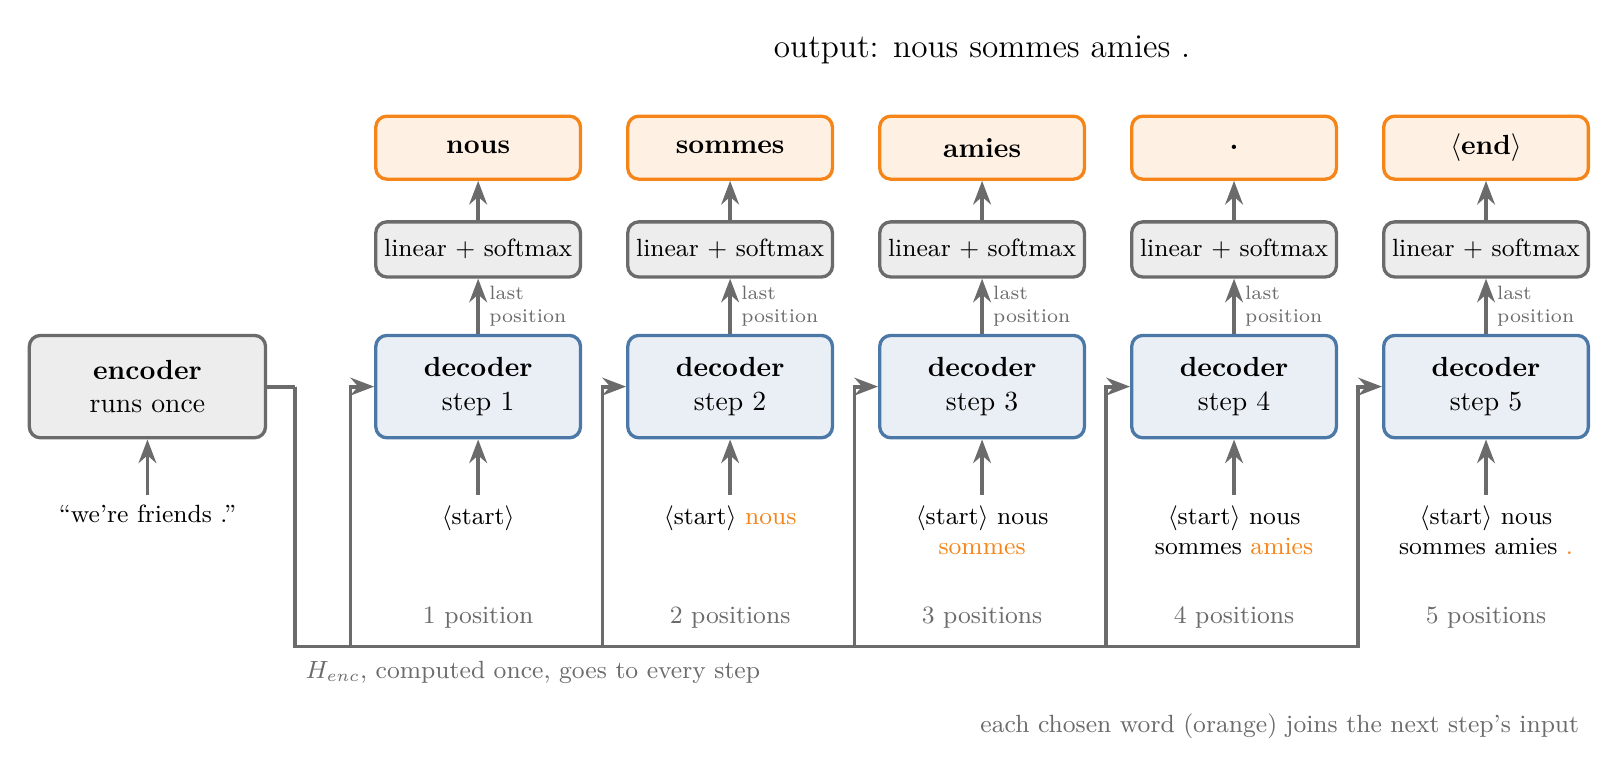
\begin{tikzpicture}[every node/.append style={font=\sffamily},
  dec/.style={box=cblue, minimum width=2.6cm, minimum height=1.3cm},
  tok/.style={font=\sffamily\small, align=center},
  outw/.style={box=corange, minimum width=2.6cm, inner sep=4pt, minimum height=0.8cm}]
  % encoder, once
  \node[box=cgrey, minimum width=3.0cm, minimum height=1.3cm] (enc) at (-4.2,0) {\textbf{encoder}\\runs once};
  \node[tok, below=0.7cm of enc] (src) {``we're friends .''};
  \draw[arrow] (src) -- (enc);
  % decoder steps
  \foreach \i/\inp/\last/\w in {1/{$\langle$start$\rangle$}/{$\langle$start$\rangle$}/nous,
                                2/{$\langle$start$\rangle$ \textcolor{corange}{nous}}/nous/sommes,
                                3/{$\langle$start$\rangle$ nous\\\textcolor{corange}{sommes}}/sommes/amies,
                                4/{$\langle$start$\rangle$ nous\\sommes \textcolor{corange}{amies}}/amies/.,
                                5/{$\langle$start$\rangle$ nous\\sommes amies \textcolor{corange}{.}}/./$\langle$end$\rangle$} {
    \node[dec] (d\i) at (3.2*\i - 3.2, 0) {\textbf{decoder}\\step \i};
    \node[tok, below=0.7cm of d\i, anchor=north] (in\i) {\inp};
    \node[note, anchor=north] at ([yshift=-2.0cm]d\i.south) {\i\ position\ifnum\i>1 s\fi};
    \draw[arrow] (in\i) -- (d\i);
    \node[box=cgrey, minimum width=2.6cm, inner sep=3pt, minimum height=0.7cm, above=0.7cm of d\i] (ls\i) {\small linear + softmax};
    \draw[arrow] (d\i) -- node[right, font=\sffamily\scriptsize, text=cgrey, align=left] {last\\position} (ls\i);
    \node[outw, above=0.5cm of ls\i] (w\i) {\textbf{\w}};
    \draw[arrow] (ls\i) -- (w\i);
  }
  % encoder output to every step: a bus below everything, risers in the gaps
  \coordinate (e0) at ([xshift=0.35cm]enc.east);
  \draw[draw=cgrey, line width=1.4pt] (enc.east) -- (e0);
  \foreach \i in {1,...,5} {
    \draw[arrow] (e0) |- ([xshift=-0.3cm, yshift=-3.3cm]d\i.west) |- (d\i.west);
  }
  \node[note, anchor=north west] at ([yshift=-3.35cm]e0) {$H_{\text{enc}}$, computed once, goes to every step};
  \node[font=\sffamily\large, above=0.5cm of w3] {output: nous sommes amies .};
  \node[note, anchor=north east] at ([yshift=-3.35cm]d5.south east) {each chosen word (orange) joins the next step's input};
\end{tikzpicture}
\end{document}
